\documentclass[a4]{article}

\usepackage[left=2cm,right=2cm,top=2cm,bottom=2cm]{geometry} 

\usepackage[utf8]{inputenc}   % otra alternativa para los caracteres acentuados y la "ñ"
\usepackage[           spanish % para poder usar el español
                      ,es-tabla % para los captions de las tablas
                       ]{babel}   
\decimalpoint %para usar el punto decimal en vez de coma para los números con decimales

%\usepackage{beton}
%\usepackage[T1]{fontenc}

\usepackage{parskip}
\usepackage{xcolor}

\usepackage{caption}

\usepackage{enumerate} % paquete para poder personalizar fácilmente la apariencia de las listas enumerativas

\usepackage{graphicx} % figuras
\usepackage{subfigure} % subfiguras

\usepackage{amsfonts}
\usepackage{amsmath}
\usepackage{listings}
\lstset{language=Python}          % Set your language (you can change the language for each code-block optionally)


\definecolor{gray}{rgb}{0.5,0.5,0.5}
\newcommand{\n}[1]{{\color{gray}#1}}
\lstset{numbers=left,numberstyle=\small\color{gray}}

\definecolor{gris}{RGB}{220,220,220}
	
\usepackage{float} % para controlar la situación de los entornos flotantes

\restylefloat{figure}
\restylefloat{table} 
\setlength{\parindent}{0mm}


\usepackage[bookmarks=true,
            bookmarksnumbered=false, % true means bookmarks in 
                                     % left window are numbered
            bookmarksopen=false,     % true means only level 1
                                     % are displayed.
            colorlinks=true,
            allcolors=blue,
            urlcolor=cyan]{hyperref}
\definecolor{webblue}{rgb}{0, 0, 0.5}  % less intense blue


\title{\Huge Inteligencia de Negocio. Práctica 3:\\
Competición de Kaggle \vspace{5mm}}

\author{\LARGE Patricia Córdoba Hidalgo \vspace{2mm}\\
  \Large patriciacorhid@correo.ugr.es \vspace{2mm}\\
  \Large Grupo 2 (Viernes) \vspace{5mm}}

\date{\today}

\begin{document}

\maketitle

\newpage
\tableofcontents
\newpage

\section{Introducción}

Nuestro problema consiste en predecir el precio de un conjunto de instancias de coches a partir de ciertas características de éste. Es un problema de aprendizaje supervisado, más concretamente de clasificación. Las etiquetas correspondientes a la variable \texttt{Precio\_cat}, aquella que queremos predecir, son las siguientes:

\begin{enumerate}
\item Coches baratos.
\item Coches menos baratos.
\item Coches con precio promedio.
\item Coches más caros que el promedio.
\item Coches muy caros.
\end{enumerate}

Las características de los coches usadas para predecir su precio son:

\begin{itemize}
\item Nombre del tipo de coche.
\item Ciudad de venta del coche.
\item Año del coche.
\item Kilómetros recorridos del coche.
\item Tipo de combustible del coche.
\item Tipo de marcha.
\item Mano (primera mano, segunda mano, tercera mano, cuarta o más).
\item Consumo.
\item CC del motor.
\item Potencia del motor.
\item Asientos del coche.
\item Descuento realizado por oferta.
\end{itemize}

Usaré distintas técnicas y modelos para predecir las etiquetas del conjunto de test. Estas etiquetas serán subidas es un fichero llamado \texttt{p3\_\{número\}.csv} a la plataforma Kaggle. La métrica usada para representar la bondad del ajuste es \textit{accuracy}.

\newpage
\section{Lista de intentos}

\begin{center}
\begin{tabular}{|c|c|c|c|c|c|c|c|}
\hline
  \multicolumn{1}{|c|}{\textbf{Archivo}} & \textbf{Fecha} & \textbf{Pos.} & \textbf{Acc. Train} & \textbf{Acc. Test} & \textbf{Preprocesado} & \textbf{Algoritmos} &\textbf{Parámetros}  \\ \hline
  
  p3\_00.csv & \begin{tabular}[c]{@{}l@{}}13:20:11\\ 20/12/20\end{tabular} & 7 & 0.826657 & 0.75237 & \begin{tabular}[c]{@{}l@{}}Eliminación de\\ la variable Descuento\\ Uso de Labelencoder\end{tabular} & Random Forest & \begin{tabular}[c]{@{}l@{}}criterion = gini\\ n\_estimators = 150\\ ccp\_alpha=0\end{tabular} \\ \hline

  p3\_01.csv & \begin{tabular}[c]{@{}l@{}}19:03:32\\ 20/12/20\end{tabular} & 4 & 0.901557 & 0.76186 & SMOTE & Random Forest & \begin{tabular}[c]{@{}l@{}}criterion = entropy\\ n\_estimators = 220\\ ccp\_alpha=0.00023\end{tabular} \\ \hline

  p3\_02.csv & \begin{tabular}[c]{@{}l@{}}15:40:15\\ 21/12/20\end{tabular} & 4 & 0.900445 & 0.75582 & \begin{tabular}[c]{@{}l@{}} Cambio de nombres\\ por marcas\end{tabular} & Random Forest & \begin{tabular}[c]{@{}l@{}}criterion = entropy\\ n\_estimators = 130\\ ccp\_alpha=0\end{tabular} \\ \hline

  p3\_04.csv & \begin{tabular}[c]{@{}l@{}}20:49:52\\ 21/12/20\end{tabular} & 2 & 0.86529 & 0.79637 & \begin{tabular}[c]{@{}l@{}} Normalización +\\ OneHotEncoder\end{tabular} & MLP & \begin{tabular}[c]{@{}l@{}}activation = tanh\\ hidden\_layer\_sizes = \\=(300,300) \\ alpha=default\end{tabular} \\ \hline

  p3\_05.csv & \begin{tabular}[c]{@{}l@{}}20:52:47\\ 21/12/20\end{tabular} & 2 & 0.881868 & 0.68162 & \begin{tabular}[c]{@{}l@{}} Normalización +\\ OneHotEncoder\end{tabular} & Knn & n\_neighbors = 1 \\ \hline

  p3\_06.csv & \begin{tabular}[c]{@{}l@{}}15:07:36\\ 22/12/20\end{tabular} & 3 & 0.920356 & 0.79982 & \begin{tabular}[c]{@{}l@{}} Normalización +\\ OneHotEncoder\end{tabular} & \begin{tabular}[c]{@{}l@{}} Gradient\\ Boosting\end{tabular} & \begin{tabular}[c]{@{}l@{}} n\_estimators = 760\\ min\_sample\_leaf = 8 \\ learning\_rate = 0.1\end{tabular} \\ \hline

  p3\_07.csv & \begin{tabular}[c]{@{}l@{}}17:25:41\\ 22/12/20\end{tabular} & 3 & 0.9330367 & 0.80241 & \begin{tabular}[c]{@{}l@{}} Normalización +\\ OneHotEncoder\end{tabular} & \begin{tabular}[c]{@{}l@{}} Stacking con \\ Gradient\\ Boosting \\ MLP y \\ Random Forest\end{tabular} & \begin{tabular}[c]{@{}l@{}} final\_estimator = \\ LogisticRegression \\con max\_iters = 400 \end{tabular} \\ \hline

  p3\_08.csv & \begin{tabular}[c]{@{}l@{}}16:53:58\\ 24/12/20\end{tabular} & 3 & 0.934805 & 0.79376 & \begin{tabular}[c]{@{}l@{}} Normalización +\\ OneHotEncoder +\\ LocalOutliersFactor \end{tabular} & \begin{tabular}[c]{@{}l@{}} Stacking con \\ Gradient\\ Boosting \\ MLP y \\ Random Forest\end{tabular} & \begin{tabular}[c]{@{}l@{}} final\_estimator = \\ LogisticRegression \\con max\_iters = 400 \end{tabular} \\ \hline

  p3\_09.csv & \begin{tabular}[c]{@{}l@{}}20:34:30\\ 24/12/20\end{tabular} & 3 & 0.9339265 & 0.80845 & \begin{tabular}[c]{@{}l@{}} Normalización +\\ OneHotEncoder \end{tabular} & \begin{tabular}[c]{@{}l@{}} Stacking con \\ Gradient\\ Boosting \\ MLP \\ Random Forest \\ y \\lightbmClassifier\end{tabular} & \begin{tabular}[c]{@{}l@{}} final\_estimator = \\ LogisticRegression \\con max\_iters = 400 \\------------\\ boosting\_type = \\ = 'goos' \\ num\_leaves = 35 \\ max\_depth = 10 \\ n\_estimators = 150 \end{tabular} \\ \hline

  p3\_10.csv & \begin{tabular}[c]{@{}l@{}}20:36:50\\ 24/12/20\end{tabular} & 1 & 0.930033 & 0.82830 & \begin{tabular}[c]{@{}l@{}} Normalización +\\ OneHotEncoder \end{tabular} & \begin{tabular}[c]{@{}l@{}} Stacking con \\ Gradient\\ Boosting \\ MLP \\ y \\lightbmClassifier\end{tabular} & \begin{tabular}[c]{@{}l@{}} final\_estimator = \\ LogisticRegression \\con max\_iters = 400 \\------------\\ boosting\_type = \\ = 'goos' \\ num\_leaves = 35 \\ max\_depth = 10 \\ n\_estimators = 150 \end{tabular} \\ \hline

\end{tabular}
\end{center}

\vspace{5mm}
NOTA: No consideré oportuno subir el fichero \texttt{p3\_03.py}, se puede considerar que ese fichero es inexistente. No es ningún error que no aparezca en la tabla de intentos.

\newpage
\section{Intentos}

\subsection{p3\_00}

Antes de nada analizamos el conjunto de training. Con la orden \texttt{datos.info()} obtenemos los atributos que componen este conjunto, el número de instancias que componen dicho conjunto y el número de valores nulos:

\begin{verbatim}
<class 'pandas.core.frame.DataFrame'>
RangeIndex: 4819 entries, 0 to 4818
Data columns (total 14 columns):
 #   Column        Non-Null Count  Dtype  
---  ------        --------------  -----  
 0   id            4747 non-null   float64
 1   Nombre        4747 non-null   object 
 2   Ciudad        4747 non-null   object 
 3   Año           4747 non-null   float64
 4   Kilometros    4747 non-null   float64
 5   Combustible   4747 non-null   object 
 6   Tipo_marchas  4747 non-null   object 
 7   Mano          4747 non-null   object 
 8   Consumo       4746 non-null   object 
 9   Motor_CC      4718 non-null   object 
 10  Potencia      4644 non-null   object 
 11  Asientos      4713 non-null   float64
 12  Descuento     659 non-null    float64
 13  Precio_cat    4819 non-null   int64  
dtypes: float64(5), int64(1), object(8)
memory usage: 527.2+ KB
\end{verbatim}

La variable Descuento posee más valores nulos que el resto, un total de 4160 valores perdidos.

Tras esto representamos el número de elementos por clase y observamos que las clases están desbalanceadas:

\begin{figure}[H]
  \centering
  \caption{Datos en cada clase}
  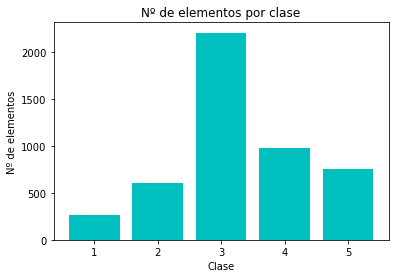
\includegraphics[width=85mm]{imagenes/count}
\end{figure}

Una vez que tenemos una idea de la distribución de los datos, pasamos a trabajar con ellos. Primero trabajamos con los valores perdidos. Si eliminásemos todos los valores perdidos, contaríamos sólo con el $11.68\%$ de los originales, con lo que perderíamos mucha información, así que descarté ese preprocesamiento.

El preprocesamiento que realicé finalmente consiste en eliminar la variable Descuento, ya que el $86.32\%$ de sus valores son perdidos y eliminar el resto de valores perdidos restantes. Esto supone quedarnos con el $81.88\%$ de los datos originales. Reorganicé los índices para que fuesen del 1 al 3945, dado que posteriormente será necesario esta numeración para recorrer el dataframe con bucles.

Esto fue realizado con el código:

\begin{lstlisting}
p2_datos = datos.copy()
del(p2_datos['Descuento'])
p2_datos = p2_datos.dropna()
p2_datos = p2_datos.reset_index()
del(p2_datos['index'])
\end{lstlisting}

Tras esto se cuantificaron todas las variables cuaitativas usando \texttt{LabelEncoder}. El \texttt{LabelEncoder} entrena con la lista total de los valores de cada atributo, que se encuentra en los ficheros \textit{.csv} correspondientes a cada uno, y se usa para transformar los datos \textit{train} y \textit{test}. De esta manera, se aplica la misma transformación en ambos.

Las variables \textit{Consumo, Motor\_CC} y \textit{Potencia} están codificadas como \texttt{string}. Para guardarlas como un \texttt{float}, eliminamos las unidades que acompañan a los valores de estas variables. Por ejemplo, el código usado para eliminar la unidad `` kmlp'' en la variable \textit{Consumo} es:

\begin{lstlisting}
for i in range(len(p2_datos)):
  p2_datos["Consumo"].iloc[i] = float(p2_datos["Consumo"].iloc[i].strip(' kmlp'))
\end{lstlisting}

Una vez preprocesados los datos, separamos las etiquetas del resto de variables:

\begin{lstlisting}
cols = [col for col in p2_datos.columns if col not in ['Precio_cat']]
data = p2_datos[cols]
del(data['id'])
target = p2_datos['Precio_cat']
\end{lstlisting}

Por último elegí el algoritmo \texttt{Random Forest} para resolver este problema y seleccioné los hiperparámetros que iba a usar. Para evaluar la bondad del modelo con cada uno de los diferentes hiperparámetros usé la media de la medida \textit{accuracy} conseguida con cada uno de los cinco conjuntos usados en validación cruzada.

Como criterio de división de nodos, usé el \texttt{gini}, ya que la accuracy media obtenida es $0.826657682373137$ mientras que con \texttt{entropy} consigue un $0.8215879738813753$.

Para elegir el número de estimadores usados, probé con diversas cantidades, obteniendo los resultados mostrados en las siguientes gráficas:

\begin{figure}[H]
  \centering
  \subfigure[Selección de \texttt{n\_stimators}]{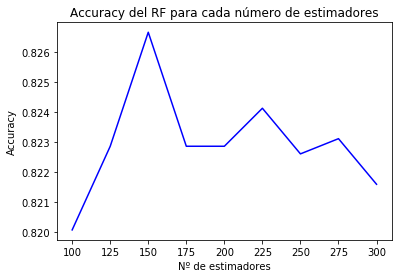
\includegraphics[width=85mm]{imagenes/p3_00_n_estimadores1}}
  \subfigure[Selección de \texttt{n\_stimators}]{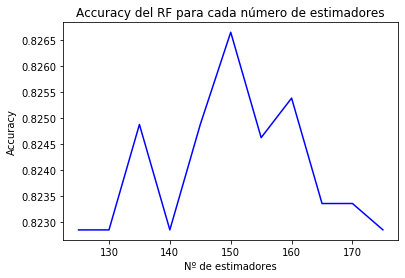
\includegraphics[width=85mm]{imagenes/p3_00_n_estimadores2}}
\end{figure}

En la primera vemos que el máximo se alcanza entorno a 150 estimadores, por lo que realicé intentos menos espaciados entorno a este número. Se aprecia que el máximo se sigue alcanzando en 150 estimadores, que es el valor por defecto de este parámetro.

También intenté identificar el parámetro de poda óptimo. Podemos comprobar que la poda empeora el desempeño del modelo, por lo que este parámetro tampoco lo modificremos.

\begin{figure}[H]
  \centering
  \caption{Selección de \texttt{ccp\_alpha}}
  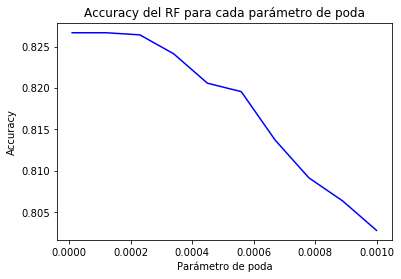
\includegraphics[width=85mm]{imagenes/p3_00_ccp_alpha}
\end{figure}

Tras todo el ajuste de hiperparámetros, el modelo final es aquel por defecto. Por tanto, para ver la \textit{accuracy} del modelo ejecutamos el siguiente código:

\begin{lstlisting}
rf_clf = RandomForestClassifier(random_state=15, n_estimators=150)
score = cross_val_score(rf_clf, data, target, cv=5)

s = 0
for i in range(len(score)):
    s+= score[i]

print("La accuracy del modelo es: " + str(s/len(score)))
\end{lstlisting}

La \textit{accuracy} del modelo en el conjunto training es: 0.826657682373137. Tras aplicar el mismo preporcesado al conjunto test, obtenemos que la \textit{accuracy} del conjunto test es 0.75237. 

\subsection{p3\_01}

En este intento, tras aplicar el preprocesamiento explicado en la prueba anterior, aplicamos SMOTE (Synthetic Minority Oversampling Technique). Con esto conseguimos que las clases estén balanceadas. El código usado para llevar esto a cabo es:

\begin{lstlisting}
data, target = SMOTE(random_state=15).fit_resample(data, target)
\end{lstlisting}

Si ejecutamos la orden \texttt{Counter(target)}, comprobamos que todas las clases tienen 1798 instancias.

Después de procesar así los datos, volvemos a ajustar los hiperparámetros del algoritmo \texttt{Random Forest}. Esta vez, el criterio de división escogido es \texttt{entropy}, que consigue una \textit{accuracy} media de $0.8997775305895438$ frente a $0.8972191323692993$ que se consigue usando \texttt{gini}. Podemos observar que la \textit{accuracy} que consigue el conjunto train con este procesamiento es mayor que sin aplicar oversampling.

Estimamos el número optimo de estimadores de igual manera que en el intento anterior:

\begin{figure}[H]
  \centering
  \subfigure[Selección de \texttt{n\_stimators}]{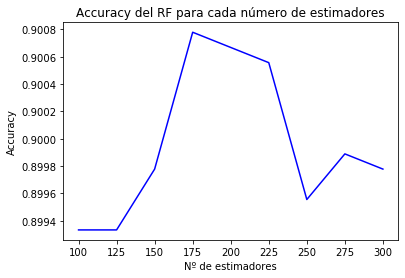
\includegraphics[width=85mm]{imagenes/p3_01_n_estimadores1}}
  \subfigure[Selección de \texttt{n\_stimators}]{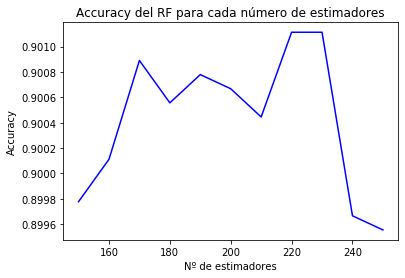
\includegraphics[width=85mm]{imagenes/p3_01_n_estimadores2}}
\end{figure}

A la vista de los resultados tomamos 220 estimadores. También estimamos el valor del parámetro de poda. Escogemos 0.00023 dados los resultados obtenidos en la siguiente gráfica:

\begin{figure}[H]
  \centering
  \caption{Selección de \texttt{ccp\_alpha}}
  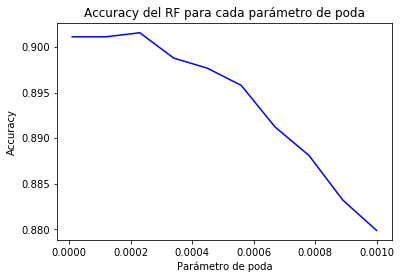
\includegraphics[width=85mm]{imagenes/p3_01_ccp_alpha}
\end{figure}

La \textit{accuracy} del modelo en el conjunto training es 0.9015572858731924. Tras aplicar el mismo preporcesado al conjunto test, obtenemos que la \textit{accuracy} del conjunto test es 0.76186.

\subsection{p3\_02}

En este intento, después de eliminar la variable Descuento y los valores nulos, y antes de usar \texttt{LableEncoder}, sustituí los nombres de los coches por las marcas de los coches usando el siguiente código:

\begin{lstlisting}
for i in range(len(nombre)):
  nombre["Nombre"].iloc[i] = nombre["Nombre"].iloc[i].split(' ')[0]

for i in range(len(p2_datos)):
    p2_datos["Nombre"].iloc[i] = p2_datos["Nombre"].iloc[i].split(' ')[0]
\end{lstlisting}

El resto del preprocesamiento se mantuvo. Volví a seleccionar los hiperparámetros del \texttt{Random Forest}:

El criterio de división elegido fue \texttt{entropy}, que consigue una \textit{accuracy} de 0.8994438264738598 frente a 0.8957730812013349 que consigue el criterio \texttt{gini}.

Seleccionamos el número de estimadores usado, que en este caso será 130, por la información representada en las siguientes gráficas:

\begin{figure}[H]
  \centering
  \subfigure[Selección de \texttt{n\_stimators}]{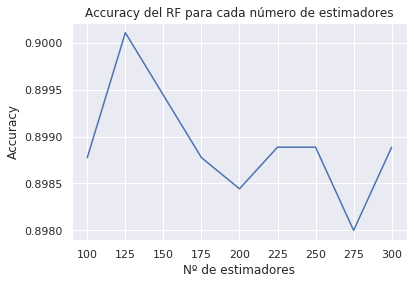
\includegraphics[width=85mm]{imagenes/p3_02_n_estimadores1}}
  \subfigure[Selección de \texttt{n\_stimators}]{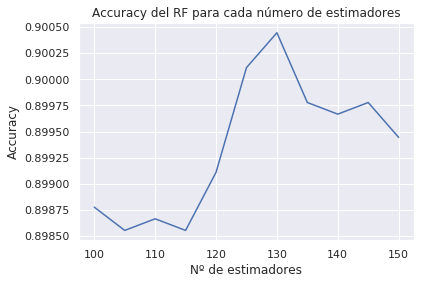
\includegraphics[width=85mm]{imagenes/p3_02_n_estimadores2}}
\end{figure}

También decidí usar el valor 0 para el parámetro de poda. El motivo se encuentra en la siguiente gráfica:

\begin{figure}[H]
  \centering
  \caption{Selección de \texttt{ccp\_alpha}}
  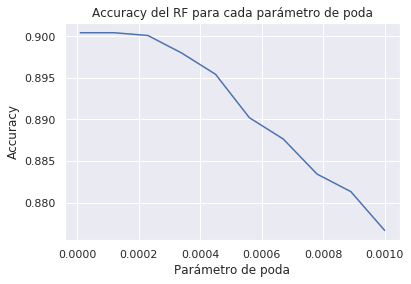
\includegraphics[width=85mm]{imagenes/p3_02_ccp_alpha}
\end{figure}


La \textit{accuracy} del modelo en el conjunto training es 0.9004449388209121. Aunque es inferior a la obtenida en el intento anterior, pensé que con este procesamiento podría reducirse el sobreajuste y obtener mejores resultados en el conjunto test. Tras aplicar el mismo preporcesado al conjunto test, obtenemos que la \textit{accuracy} del conjunto test es 0.75582, por tanto mis sospechas no eran ciertas.

\subsection{p3\_04}

En este intento quise probar con un modelo diferente, \texttt{MLP}. Este modelo requiere un preprocesado diferente, ya que la normalización y el uso de \texttt{OneHotVectors} hace que el modelo obtenga mejores resultados.

El procesamiento usado en esta prueba consiste entonces en eliminar, como en las anteriores, la variable Descuento y los valores nulos restantes. Luego pasamos los nombres de los coches a marcas, del mismo modo que hicimos en \texttt{p3\_02}, para reducir así el número de variables finales (habrá una variable por cada posible valor del atributo cualitativo al que apliquemos \texttt{OneHotEncoder}).

En vez de aplicar \texttt{LabelEncoder} a las variables cualitativas, usé \texttt{OneHotEncoder}. Esto nos crea una nueva variable por cada uno de los posibles valores que tomase la variable a la que se lo aplicamos. Añadimos estas variables al \texttt{DataFrame} de datos y eliminamos la variable original.

Un ejemplo del código usado para esto es:

\begin{lstlisting}
encCiudad = OneHotEncoder(handle_unknown='ignore')
encCiudad.fit(ciudad["Ciudad"].to_numpy().reshape(-1, 1))
aux = encCiudad.transform(p2_datos["Ciudad"].to_numpy().reshape(-1, 1)).toarray()
aux = pd.DataFrame(aux)

for i in range(aux.shape[1]):
    p2_datos["Ciudad " + str(i)] = aux[i]
    
del(p2_datos['Ciudad'])
\end{lstlisting}

Tras esto, volvemos a eliminar las unidades de las variables \textit{Consumo, Motor\_CC} y \textit{Potencia} como se explicó en \texttt{p3\_00} y así pasar a \texttt{float} sus valores.

La estructura de los datos es ahora:

\begin{verbatim}
<class 'pandas.core.frame.DataFrame'>
RangeIndex: 3946 entries, 0 to 3945
Data columns (total 61 columns):
 #   Column          Non-Null Count  Dtype  
---  ------          --------------  -----  
 0   id              3946 non-null   float64
 1   Año             3946 non-null   float64
 2   Kilometros      3946 non-null   float64
 3   Consumo         3946 non-null   float64
 4   Motor_CC        3946 non-null   float64
 5   Potencia        3946 non-null   float64
 6   Asientos        3946 non-null   float64
 7   Precio_cat      3946 non-null   int64  
 8   Nombre 0        3946 non-null   float64
 9   Nombre 1        3946 non-null   float64
 10  Nombre 2        3946 non-null   float64
 11  Nombre 3        3946 non-null   float64
 12  Nombre 4        3946 non-null   float64
 13  Nombre 5        3946 non-null   float64
 14  Nombre 6        3946 non-null   float64
 15  Nombre 7        3946 non-null   float64
 16  Nombre 8        3946 non-null   float64
 17  Nombre 9        3946 non-null   float64
 18  Nombre 10       3946 non-null   float64
 19  Nombre 11       3946 non-null   float64
 20  Nombre 12       3946 non-null   float64
 21  Nombre 13       3946 non-null   float64
 22  Nombre 14       3946 non-null   float64
 23  Nombre 15       3946 non-null   float64
 24  Nombre 16       3946 non-null   float64
 25  Nombre 17       3946 non-null   float64
 26  Nombre 18       3946 non-null   float64
 27  Nombre 19       3946 non-null   float64
 28  Nombre 20       3946 non-null   float64
 29  Nombre 21       3946 non-null   float64
 30  Nombre 22       3946 non-null   float64
 31  Nombre 23       3946 non-null   float64
 32  Nombre 24       3946 non-null   float64
 33  Nombre 25       3946 non-null   float64
 34  Nombre 26       3946 non-null   float64
 35  Nombre 27       3946 non-null   float64
 36  Nombre 28       3946 non-null   float64
 37  Nombre 29       3946 non-null   float64
 38  Nombre 30       3946 non-null   float64
 39  Ciudad 0        3946 non-null   float64
 40  Ciudad 1        3946 non-null   float64
 41  Ciudad 2        3946 non-null   float64
 42  Ciudad 3        3946 non-null   float64
 43  Ciudad 4        3946 non-null   float64
 44  Ciudad 5        3946 non-null   float64
 45  Ciudad 6        3946 non-null   float64
 46  Ciudad 7        3946 non-null   float64
 47  Ciudad 8        3946 non-null   float64
 48  Ciudad 9        3946 non-null   float64
 49  Ciudad 10       3946 non-null   float64
 50  Combustible 0   3946 non-null   float64
 51  Combustible 1   3946 non-null   float64
 52  Combustible 2   3946 non-null   float64
 53  Combustible 3   3946 non-null   float64
 54  Combustible 4   3946 non-null   float64
 55  Tipo_marchas 0  3946 non-null   float64
 56  Tipo_marchas 1  3946 non-null   float64
 57  Mano 0          3946 non-null   float64
 58  Mano 1          3946 non-null   float64
 59  Mano 2          3946 non-null   float64
 60  Mano 3          3946 non-null   float64
dtypes: float64(60), int64(1)
memory usage: 1.8 MB
\end{verbatim}

Como vemos, ahora hay 61 variables en vez de 13 (14 menos el Descuento) y no hay valores nulos.

Por último, normalizamos los datos de las variables cuantitativas usando \texttt{MinMaxScaler}. Como siempre, entrenamos con el archivo con los posibles valores de la variable y luego aplicamos la misma transformación a los datos training y test. Un  ejemplo del código usado para normalizar es:

\begin{lstlisting}
scalerKilometros = MinMaxScaler()
scalerKilometros.fit(kilometros["Kilometros"].to_numpy().reshape(-1, 1))
aux = scalerKilometros.transform(p2_datos["Kilometros"].to_numpy().reshape(-1, 1))
aux = pd.DataFrame(aux)
p2_datos["Kilometros"] = aux[0]
\end{lstlisting}

Una vez hecho esto, separamos los datos de las etiquetas, aplicamos oversampling y ajustamos los hiperparámetros de \texttt{MLP}. Para esste algoritmo, el parámetro que estimamos es \texttt{hidden\_layer\_sizes}.

\begin{figure}[H]
  \centering
  \caption{Selección de \texttt{hidden\_layer\_sizes}}
  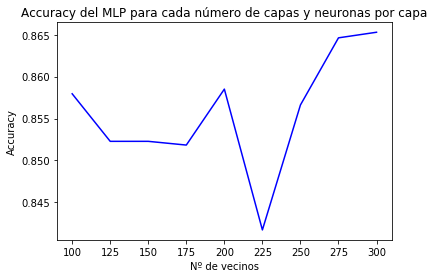
\includegraphics[width=85mm]{imagenes/p3_04_layers}
\end{figure}

La \textit{accuracy} del modelo en el conjunto training es 0.8652947719688543. Tras aplicar el mismo preporcesado al conjunto test, obtenemos que la \textit{accuracy} del conjunto test es 0.79637.

\subsection{p3\_05}

En este intento usé el mismo preprocesamiento de datos que en el anterior, pero el modelo que entrené fue \texttt{K-nn}. Ajustamos el parámetro \texttt{n\_neighbors}, obteniendo que el valor óptimo es 1.


\begin{figure}[H]
  \centering
  \caption{Selección de \texttt{n\_neighbors}}
  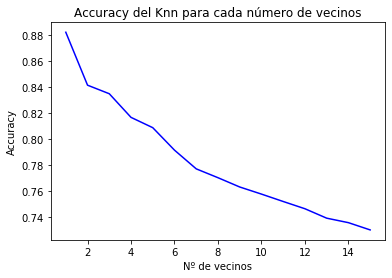
\includegraphics[width=85mm]{imagenes/p3_05_vecinos}
\end{figure}

La \textit{accuracy} del modelo en el conjunto training es 0.8818687430478309, superior a la obtenida con \texttt{MLP}. Sin embargo, tras aplicar el mismo preporcesado al conjunto test, obtenemos que la \textit{accuracy} del conjunto test es 0.68162, el peor resultado obtenido.

\subsection{p3\_06}

Con el mismo preprocesamiento usado en \texttt{p3\_04} entrenamos el algoritmo \texttt{Gradient Boosting}. El primer parámetro que seleccionamos es \texttt{n\_stimators}. Al igual que con \texttt{Random Forest} hacemos primero una visión global del comportamiento del algoritmo dependiendo de este parámetro y luego hacemos ejecuciones con valores menos espaciados entorno al máximo encontrado. A la vista de los resultados, escogemos el valor 760 para este parámetro.

\begin{figure}[H]
  \centering
  \subfigure[Selección de \texttt{n\_stimators}]{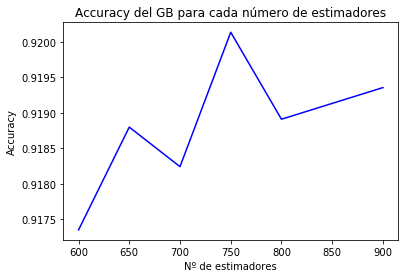
\includegraphics[width=87mm]{imagenes/p3_06_n_estimadores1}}
  \subfigure[Selección de \texttt{n\_stimators}]{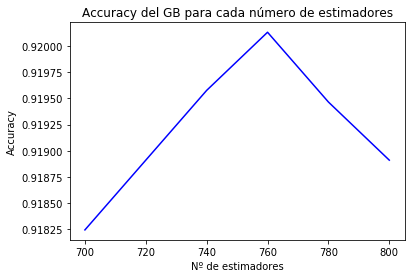
\includegraphics[width=87mm]{imagenes/p3_06_n_estimadores2}}
\end{figure}

\newpage
Buscamos también el valor óptimo para el parámetro \texttt{min\_samples\_leaf} y observamos que obtenemos los valores máximos de \textit{accuracy} en 1 y en 8. Elegí el valor 8 porque al exigir mayor número de muestras por nodo, evitas nodos con muy pocas muestras y así se puede reducir el sobreajuste.

\begin{figure}[H]
  \centering
  \caption{Selección de \texttt{min\_samples\_leaf}}
  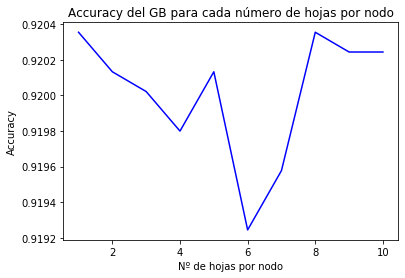
\includegraphics[width=85mm]{imagenes/p3_06_n_hojas}
\end{figure}



\end{document}
